\documentclass[14pt,a4paper]{article}

% =================== PACOTES ===================
\usepackage[utf8]{inputenc}
\usepackage[T1]{fontenc}
\usepackage[brazil]{babel}
\usepackage{graphicx}   % para inserir o logo
\usepackage{setspace}   % espaçamento
\usepackage{geometry}   % margens
\usepackage{tcolorbox}  % caixas de solução
\usepackage{fancyhdr}   % cabeçalho e rodapé
\usepackage{float}
\usepackage{caption}
\tcbuselibrary{theorems}

\geometry{a4paper, top=3cm, bottom=2.5cm, left=3cm, right=2.5cm}

% =================== CABEÇALHO ===================
\pagestyle{fancy}
\fancyhf{}
\fancyhead[L]{Maykon Hopka -- 23203081}  
\fancyfoot[C]{\thepage}

% =================== AMBIENTE DE SOLUÇÃO ===================
\newtcbtheorem[number within=section]{solucao}{Solução}%
{colback=green!5,colframe=green!60!black,fonttitle=\bfseries}{sol}

% =================== CAPA ===================
\begin{document}
\begin{titlepage}
    \centering
    
    % Logo UFSC (precisa ter o arquivo logo_ufsc.png na pasta)
    
\includegraphics[width=0.25\textwidth]{logo_ufsc.png}\par\vspace{1cm}
    
    {\Large\bfseries Universidade Federal de Santa Catarina \par}
    \vspace{0.5cm}
    {\large Centro de Engenharias da Mobilidade \par}
    {\large Curso de Engenharia Mecatrônica \par}
    \vfill
    
    {\Huge\bfseries Exercício de Threads \par}
    \vspace{0.5cm}
    {\Large Disciplina: Sistemas Operacionais\par}
    \vspace{0.3cm}
    {\large Aluno: Maykon Hopka \par}
    \vfill
    
    {\large Joinville – 2025}
\end{titlepage}

% =================== CONTEÚDO ===================
\section{Exercícios}

\subsection*{Exercício 1}
Pesquise sobre a função \texttt{pthread\_join} e explique o que ela faz.

\begin{solucao}{Exercício 1}{}
A função \texttt{pthread\_join} serve para **sincronizar threads**,  
ou seja, faz a thread chamadora esperar até que a thread especificada termine. 
\end{solucao}

\subsection*{Exercício 2}

Implemente um programa que calcule a soma dos valores contidos em um vetor de tamanho $N$ utilizando \textit{threads}.

\begin{enumerate}
    \item Divida a tarefa de cálculo proporcionalmente entre o número de \textit{threads} criadas, garantindo que cada \textit{thread} acesse apenas a sua parte do vetor, sem sobreposição.
    \item Meça o tempo de execução do programa utilizando o comando \texttt{time} no terminal.
    \item Analise os resultados obtidos e discuta se houve ganho de desempenho ao utilizar múltiplas \textit{threads} em comparação à execução com uma única \textit{thread}.
\end{enumerate}

% --- INÍCIO DA SOLUÇÃO DO EXERCÍCIO 2 ---
    \begin{center}
        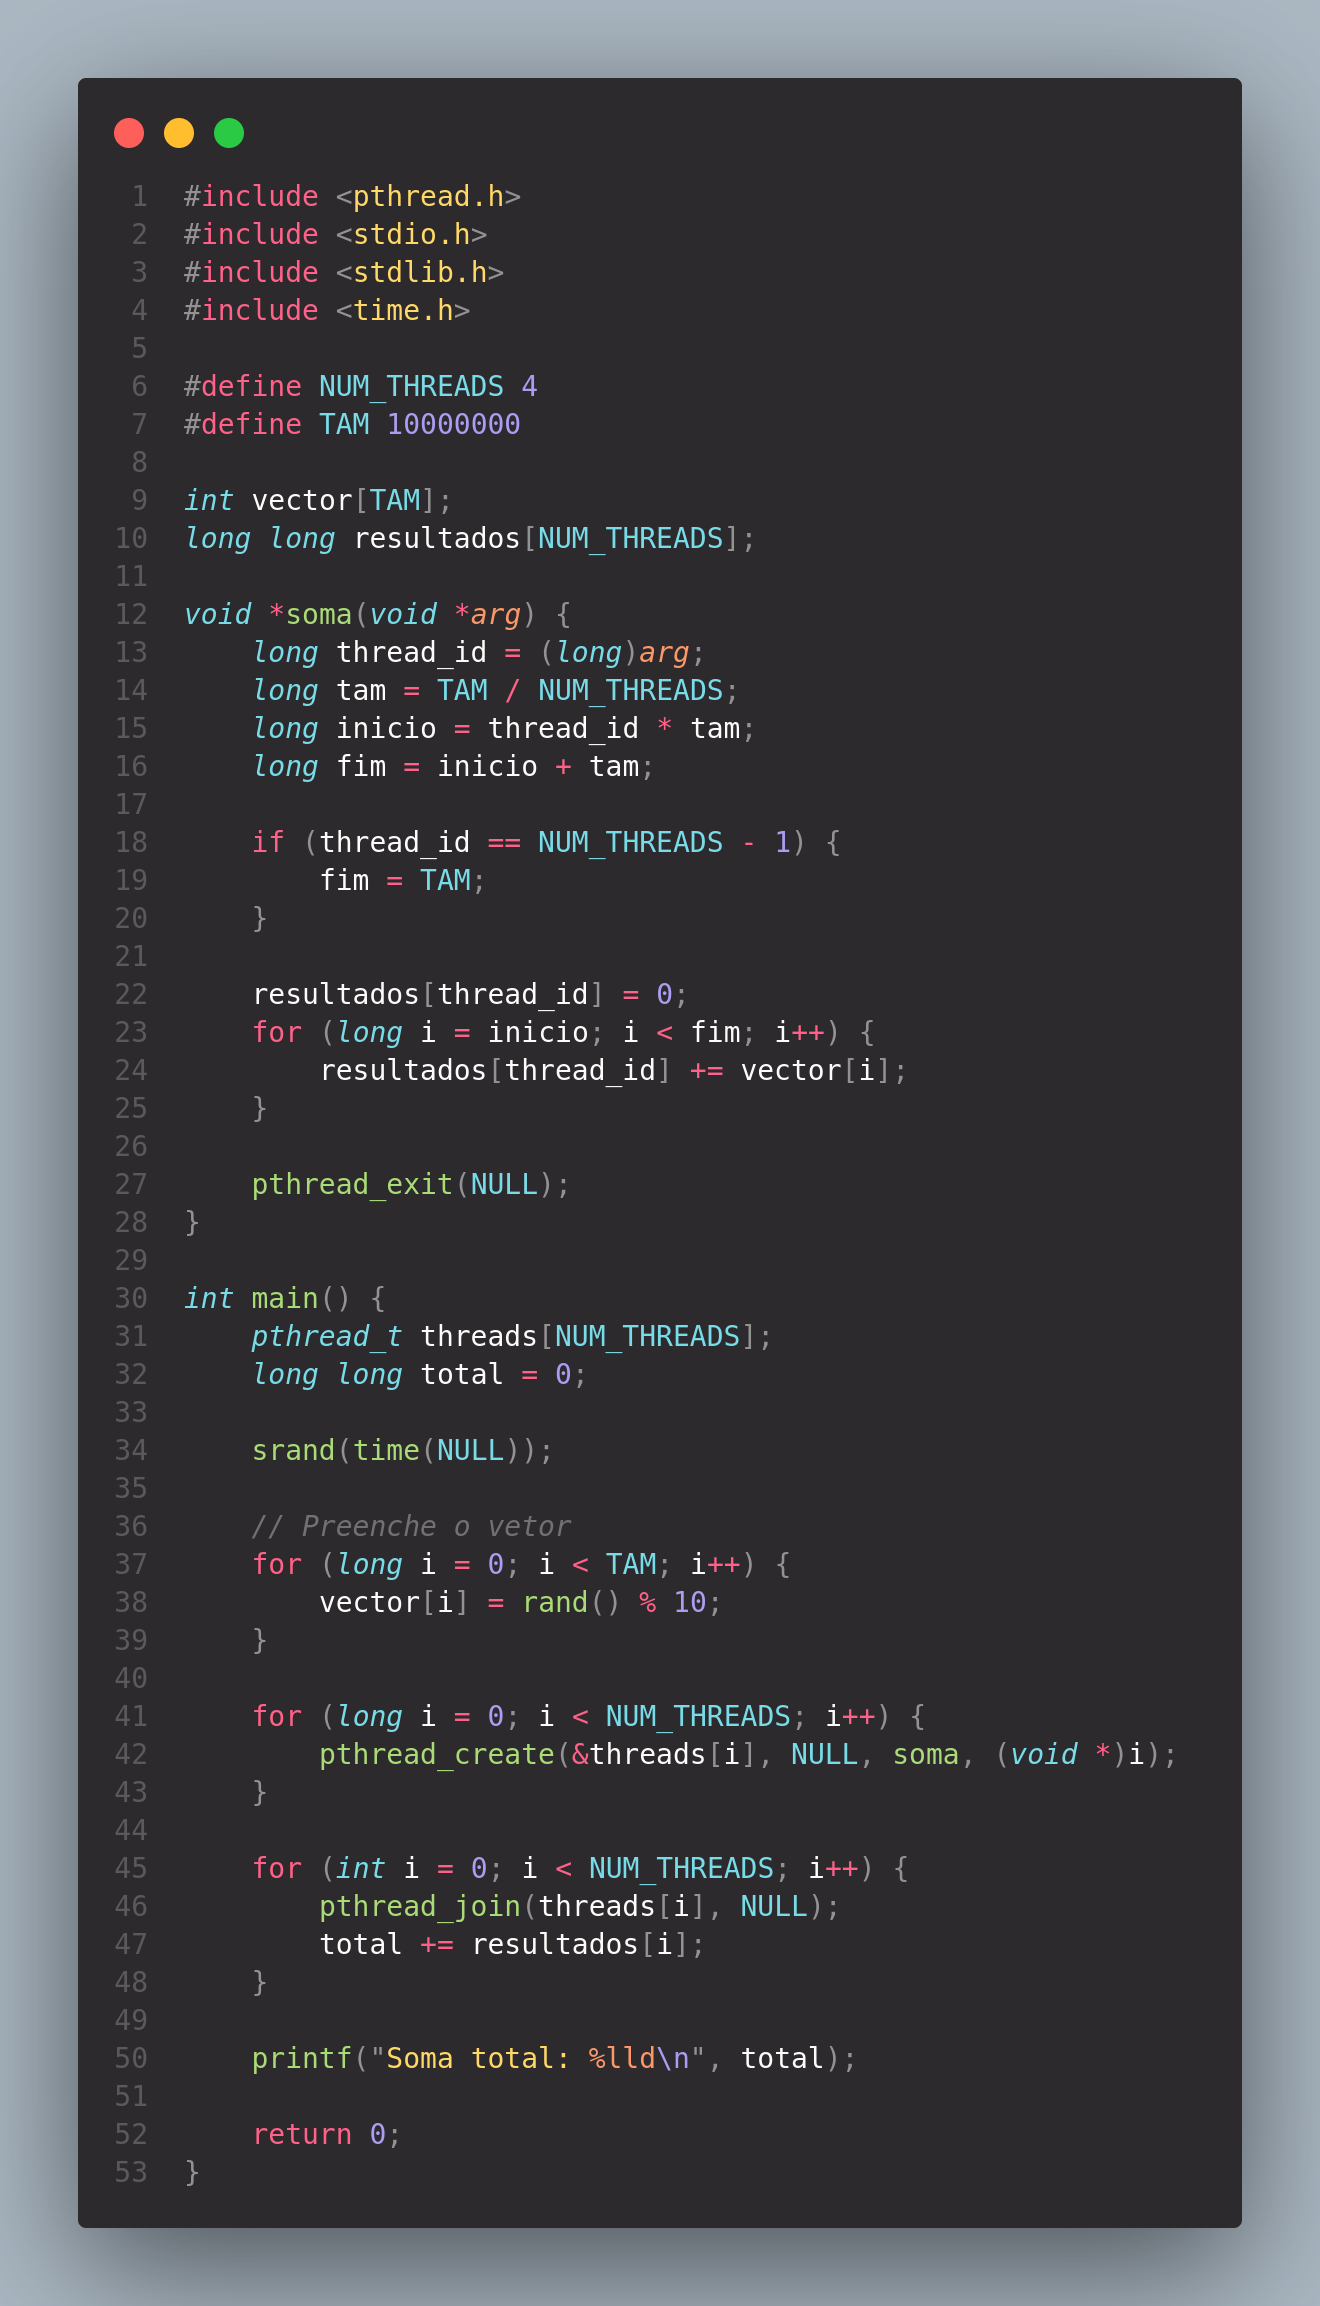
\includegraphics[width=0.5\textwidth]{code.png}
        \captionof{figure}{}
    \end{center}

    \paragraph{1. Medição do Tempo de Execução:}O comando \texttt{time} foi utilizado para medir a execução da versão sequencial (\texttt{./soma}) e da versão paralela (\texttt{./thread}).

    \textbf{Execução Sequencial (1 thread):}
    \begin{verbatim}
$ time ./soma
Soma total: 2250037019
./soma  6,84s user 0,43s system 99% cpu 7,270 total
    \end{verbatim}

    \textbf{Execução Paralela (4 threads):}
    \begin{verbatim}
$ time ./thread
Soma total: 2250000642
./thread  9,20s user 0,42s system 133% cpu 7,213 total
    \end{verbatim}

    \paragraph{2. Análise:} 

    \begin{itemize}
        \item Tempo Sequencial ($T_s$): $7,270$ segundos.
        \item Tempo Paralelo ($T_p$): $7,213$ segundos.
    \end{itemize}
    $$ \text{Ganho \%} = \left( \frac{T_s - T_p}{T_s} \right) \times 100 = \left( \frac{7,270 - 7,213}{7,270} \right) \times 100 \approx 0,78\% $$
    A implementação paralela foi aproximadamente \textbf{0,78\% mais rápida}.

    \subparagraph{Análise do Uso de CPU:} Apesar de não se mostrar muito mais rápido temos a certeza que está utilizando mais de um núcleo pois:
    \begin{itemize}
        \item \textbf{99\% cpu (Sequencial):} Um processo de thread única está limitado a um único núcleo. O valor de 99\% confirma que o programa utilizou a capacidade máxima de \textbf{um núcleo} de processador.
        \item \textbf{133\% cpu (Paralelo):} Um valor superior a 100\% é a prova de que o sistema operacional alocou as threads do processo para execução em \textbf{mais de um núcleo simultaneamente}. 
    \end{itemize}
% --- FIM DA SOLUÇÃO DO EXERCÍCIO 2 ---

\newpage



\end{document}